\section{Ontwerpen}
\label{sec:Ontwerpen}
Tijdens het ontwerpen wordt er gebruikgemaakt van UML.
Er zullen verschillende UML diagrammen gemaakt worden op basis van het 4 + 1 view model \Parencite{4+1Model} .
Dit wordt gerealiseerd na het onderzoek wanneer de requirements bekend zijn.
In figuur \ref{fig:4+1Model} wordt beschreven welke diagrammen in theorie gebruikt kunnen worden voor de verschillende views van het 4 + 1 view model.\\
\begin{graphic}
    \vspace{0.2cm}
    \captionsetup{type=figure}
    \caption{Verschillende UML diagrammen die mogelijk gebruikt kunnen worden bij de verschillende views \Parencite{4p1ModelViews}}
    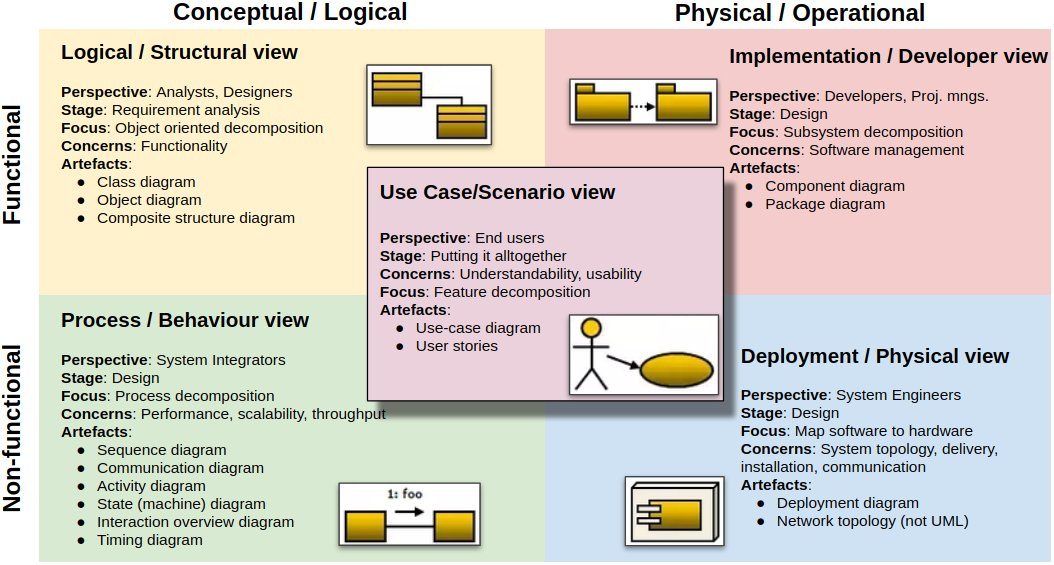
\includegraphics[scale=0.4]{4p1ModelViews}
    \label{fig:4+1Model}
    \vspace{0.2cm}
\end{graphic}
